\documentclass[11pt,a4paper]{article}
\usepackage[utf8]{inputenc}
\usepackage[english]{babel}
\usepackage{amsmath}
\usepackage{amsfonts}
\usepackage{amssymb}
\usepackage{graphicx}
\graphicspath{{../figures/}}
\author{Jacob Heden Malm}
\title{DD2424 Assignment 2}
\begin{document}
\maketitle

\section{Analytic gradient computations}
Since I wrote my code in python I could not use the provided ComputeGradsNum() method. Instead I performed the sanity check as specified in the lab instructions to check that my gradient computations were correct. I wrote a method called sanity\_check() where I passed in 100 data points and attempted to get my loss values as low as possible. I did this by training on the entire batch of data passed in for 1000 epochs and monitoring the development of the loss values.\\

Here is an example of the development of the loss values through training on this very limited data set.

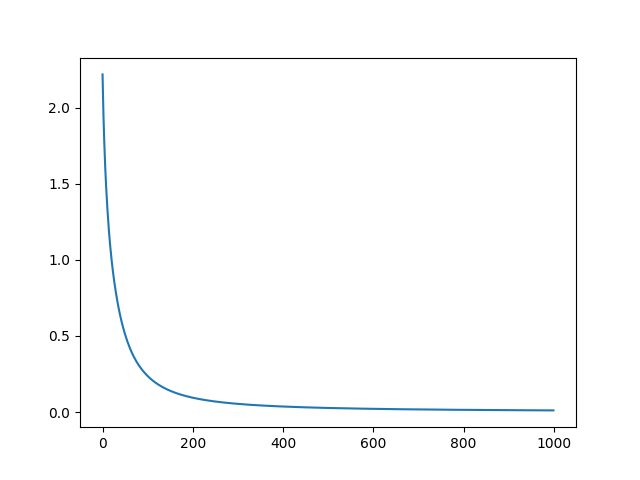
\includegraphics[width=\textwidth]{sanity_check.png}

The shape of the development is almost exactly what we'd expect, and we also manage to get almost arbitrarily close to 0, suggesting that the network learns to recognize the training set perfectly, which allows us to conclude that the gradient computations are in fact working.


best network param final accuracy: 0.5263333333333333
\end{document}
